\documentclass[10pt]{article}\usepackage[]{graphicx}\usepackage[]{color}
%% maxwidth is the original width if it is less than linewidth
%% otherwise use linewidth (to make sure the graphics do not exceed the margin)
\makeatletter
\def\maxwidth{ %
  \ifdim\Gin@nat@width>\linewidth
    \linewidth
  \else
    \Gin@nat@width
  \fi
}
\makeatother

\definecolor{fgcolor}{rgb}{0.345, 0.345, 0.345}
\newcommand{\hlnum}[1]{\textcolor[rgb]{0.686,0.059,0.569}{#1}}%
\newcommand{\hlstr}[1]{\textcolor[rgb]{0.192,0.494,0.8}{#1}}%
\newcommand{\hlcom}[1]{\textcolor[rgb]{0.678,0.584,0.686}{\textit{#1}}}%
\newcommand{\hlopt}[1]{\textcolor[rgb]{0,0,0}{#1}}%
\newcommand{\hlstd}[1]{\textcolor[rgb]{0.345,0.345,0.345}{#1}}%
\newcommand{\hlkwa}[1]{\textcolor[rgb]{0.161,0.373,0.58}{\textbf{#1}}}%
\newcommand{\hlkwb}[1]{\textcolor[rgb]{0.69,0.353,0.396}{#1}}%
\newcommand{\hlkwc}[1]{\textcolor[rgb]{0.333,0.667,0.333}{#1}}%
\newcommand{\hlkwd}[1]{\textcolor[rgb]{0.737,0.353,0.396}{\textbf{#1}}}%

\usepackage{framed}
\makeatletter
\newenvironment{kframe}{%
 \def\at@end@of@kframe{}%
 \ifinner\ifhmode%
  \def\at@end@of@kframe{\end{minipage}}%
  \begin{minipage}{\columnwidth}%
 \fi\fi%
 \def\FrameCommand##1{\hskip\@totalleftmargin \hskip-\fboxsep
 \colorbox{shadecolor}{##1}\hskip-\fboxsep
     % There is no \\@totalrightmargin, so:
     \hskip-\linewidth \hskip-\@totalleftmargin \hskip\columnwidth}%
 \MakeFramed {\advance\hsize-\width
   \@totalleftmargin\z@ \linewidth\hsize
   \@setminipage}}%
 {\par\unskip\endMakeFramed%
 \at@end@of@kframe}
\makeatother

\definecolor{shadecolor}{rgb}{.97, .97, .97}
\definecolor{messagecolor}{rgb}{0, 0, 0}
\definecolor{warningcolor}{rgb}{1, 0, 1}
\definecolor{errorcolor}{rgb}{1, 0, 0}
\newenvironment{knitrout}{}{} % an empty environment to be redefined in TeX

\usepackage{alltt}
% !Rnw weave = knitr
%% \VignetteIndexEntry{An overview of psd}
%% \VignetteEngine{knitr}
%
\usepackage[T1]{fontenc}
\usepackage[utf8]{inputenc}
\usepackage{fancyvrb}
\usepackage[pdfborder={0 0 0}]{hyperref}
\usepackage{url}
\usepackage{upquote}
\usepackage{graphicx}
\usepackage{grffile}
\usepackage{float}
\usepackage{natbib}
\usepackage{amsmath}
\usepackage{geometry}
\geometry{verbose,tmargin=3cm,bmargin=5cm,lmargin=2.5cm,rmargin=2.5cm}
\usepackage[font=sf, labelfont={sf,bf}, margin=2cm]{caption}
\usepackage{color}
\usepackage{txfonts}
%
\newcommand{\SC}[1]{\textsc{#1}}
\newcommand{\SCY}[0]{\SC{Yes}}
\newcommand{\SCN}[0]{\SC{No}}
\newcommand{\Rcmd}[1]{\texttt{#1}}
\newcommand{\psd}[0]{\href{http://www.github.com/abarbour/psd/}{\color{blue}\Rcmd{psd}}}
%
\title{An overview of \psd{}: Adaptive sine multitaper power spectral density estimation in R}
\author{Andrew J. Barbour and Robert L. Parker}
%
\IfFileExists{upquote.sty}{\usepackage{upquote}}{}
\begin{document}
\maketitle

\begin{abstract}
  This vignette provides an overview of some 
  features included in the package \psd{}, designed to
  compute estimates of power spectral
  density (PSD) for a univariate series in a sophisticated manner,
  with very little tuning effort.
  The sine multitapers are used, and
  the number of tapers varies with spectral shape, according
  to the optimal value proposed by \citet{rs1995}.
  The adaptive procedure
  iteratively refines the optimal number of tapers at each frequency
  based on the spectrum from the previous iteration.
  Assuming the adaptive procedure converges, 
  this produces power spectra
  with significantly
  lower spectral variance 
  relative to results from less-sophisticated estimators.
  Sine tapers exhibit excellent
  leakage suppression characteristics, so bias effects
  are also reduced.
  Resolution and uncertainty vary with the number of tapers,
  which means we do
  not need to resort to either (1) windowing methods,
  which inherently degrade resolution at low-frequency
  (e.g. Welch's method); or (2) smoothing kernels,
  which can badly distort important features without careful tuning
  (e.g. the Daniell kernel in \Rcmd{stats::spectrum}).
  In this regards
  \psd{} is best suited for data having 
   large dynamic range and some mix of narrow and wide-band structure,
   features typically found in geophysical datasets.
\end{abstract}

\tableofcontents
\clearpage


%opts_knit$set(verbose = TRUE)

\section{Quick start: A minimal example.}
First, we load the package into the namespace:
%% libload
\input{figure/Load_library_.tex}
For a series to analyze, we can use \Rcmd{magnet}, included in \psd{},
which represents along-track measurements
of horizontal magnetic-field strength from a gimbaled, airborne magnetometer.
These data are a small subset of the full Project MAGNET series \citep{coleman1992},
which has provided insight into
the history of the Earth's oceanic crust 
\citep{parker1997, obrien1999, korte2002}.
The sampling interval is
once every kilometer (km), so the data will represent
crustal magnetization with wavelengths longer than 2 km.
%% Project MAGNET data
\input{figure/Load_Project_MAGNET_data_.tex}
The format of the data set is a \Rcmd{data.frame} with four
sets of information:
%%
\input{figure/Show_contents_of_Project_MAGNET_.tex}
The \Rcmd{raw} and \Rcmd{clean} names represent raw
and edited intensities respectively, expressed in units of nanotesla; 
\Rcmd{mdiff} is the difference between them.
The difference between them is a matter of just a few points
attributable to instrumental malfunction; but, as we will see, the
outliers adversely affect the accuracy of any type PSD estimate, regardless
of the level of sophistication of the method.
%%
\input{figure/Outliers_.tex}
\input{figure/Outliers.tex}

We can find power spectral density (PSD)
estimates for the two series quite simply with \Rcmd{pspectrum}:
%%
\input{figure/MAGPSDS.tex}
Each application of \Rcmd{pspectrum} calculates a pilot PSD, followed by 
\Rcmd{niter}
iterations of refinement.
With each iteration
the number of tapers is adjusted 
based on the proposed optimal number from \citet{rs1995}, which
depends on spectral shape; we use 
quadratically weighted spectral derivatives \citep{prieto2007}
to estimate this shape.
Note that if the user forgets to assign the results of
\Rcmd{pspectrum} to the global environment, the result can
be recovered with the \Rcmd{psd\_envGet} function:
%%
\input{figure/FINALPSDS.tex}

In general, spectral variance is reduced
with sequential refinements\footnote{
  Messages are given by default; ones which read
  ``Ave. S.V.R." are in reference to 
  average spectral-variance reduction, which
  we define here as the variance of the
  double-differenced spectra at each stage, relative
  to the spectral variance in the pilot estimate.
}, but is not necessarily guaranteed to reduce monotonically.

Figure \ref{fig:pmag} compares power spectra for the \Rcmd{raw} and \Rcmd{clean} 
series produced by \Rcmd{stats::spectrum} and \Rcmd{pspectrum}\footnote{
  Note that \Rcmd{pspectrum} returns an object with class \Rcmd{spec} (and \Rcmd{amt}), so 
  we have access to methods within \Rcmd{stats}, including \Rcmd{plot.spec}.
} using default settings.
%
We expect the Project MAGNET data to be linear in the space of
linear-frequencies and logarithmic-power; in fact there is a clear
improvement in spectral shape between the two series,
simply because the large outliers have been removed.
%
The PSD of the clean series shows the type of spectrum typical of 
geophysical processes \citep{agnew1992}, and a rolloff in signal
for 10 kilometer wavelengths and longer; whereas, the 
PSD for the raw series looks somewhat unrealistic at shorter wavelengths -- features 
which could be difficult to judge with high spectral variance.

\begin{figure}[!htbp]
\begin{center}
\input{figure/RAWvCLEAN.tex}
\caption{Power spectral density estimates for the raw and cleaned
         Project MAGNET data bundled with \psd{}: see \Rcmd{?magnet}. 
         Points are estimates produced by \Rcmd{spectrum} and
         dashed lines are estimates produced by \Rcmd{pspectrum}, using the
         default settings.
         \emph{Note that because the objects class includes \Rcmd{`spec'}, we have
         utilized existing methods in the \Rcmd{stats} namespace. The bandwidth
         and confidence interval estimates are for the \Rcmd{spectrum}-based result.}
}
\label{fig:pmag}
\end{center}
\end{figure}

\clearpage

\section{Comparisons with other methods}

As we have shown in the Project MAGNET example, a more accurate estimate
of the power spectrum can help improve understanding of the physics 
behind the signals in the data.
But, assuming a sample is free of non-physical points, how do
PSD estimates from \psd{} compare with other methods?
Unfortunately the suite of extensions with similar functionality
is relatively limited, but hopefully we have
summarized most, if not all, the available functions in Table \ref{tbl:methods}.

%%
%% for use in psd_overview.
%%
\begin{table}[htbp!]
\begin{centering}

\caption{A comparison of power spectral density estimators in R,
excluding extensions which only estimate raw-periodograms.
Normalizations are shown as either ``single" or ``double" for
either single- or double-sided spectra, and ``various"
if there are multiple, optional normalizations. A $(*)$ denotes
the default for a function having an option for 
either single or double.
}

\begin{tabular}{r l c c c l}
\hline
\SC{Function} & \SC{Namespace} & \SC{Sine m.t.?} & \SC{Adaptive?} & \SC{Norm.} & \SC{Reference} \\
\hline
\Rcmd{bspec}     & \Rcmd{bspec}     & \SCN{} & \SCN{} & single$^*$ & \citet{rover2011} \\
\Rcmd{mtapspec}  & \Rcmd{RSEIS}     & \SCY{} & \SCN{} & various & \citet{lees1995} \\
\Rcmd{pspectrum} & \psd{}           & \SCY{} & \SCY{} & single  & \citet{barbour2014,psdR} \\
\Rcmd{spectrum}  & \Rcmd{stats}     & \SCN{} & \SCN{} & double  & \citet{rcore} \\
\Rcmd{spec.mtm}  & \Rcmd{multitaper}& \SCY{} & \SCY{} & double & \citet{rahim2012} \\
\Rcmd{SDF}       & \Rcmd{sapa}      & \SCY{} & \SCN{} & single$^*$ & \citet{percival1993} \\
\hline
\end{tabular}
\label{tbl:methods}
\end{centering}
\end{table}


We compare results from
\psd{} with those from a few of the methods in Table \ref{tbl:methods},
using the same data: the cleaned Project MAGNET series.

%%
%% spectrum
%%
\subsection{\Rcmd{stats::spectrum}}

Included in the core distribution of R is \Rcmd{stats::spectrum}, which
accesses \Rcmd{stats::spec.ar} or \Rcmd{stats::spec.pgram} (which was used
for the estimates in Figure \ref{fig:pmag}) for either
parametric and non-parametric estimation, respectively.  
The user can optionally apply a single cosine taper, and/or a smoothing kernel.
Our method is non-parametric; hence, we will compare to the latter.

Included in \Rcmd{psdcore} is an option to compare the 
results with cosine-tapered periodogram,
found with a command equivalent to this:
\input{figure/Naive_spectrum_estimation.tex}
Within \Rcmd{psdcore} the comparison is made with the logical argument \Rcmd{preproc} 
passed to \Rcmd{spec.pgram}, which is \SC{True} by default.

As a matter of bookkeeping and good practice, we should consider the working environment
accessed by \psd{} functions. 
To ensure \Rcmd{psdcore} does not access any inappropriate information leftover
from the previous calculations, we can set \Rcmd{refresh=TRUE}; we then 
re-calculate the multitaper PSD and the raw periodogram with \Rcmd{plotpsd=TRUE}; these
results are shown in Figure \ref{fig:two}.

\begin{figure}[!htbp]
\begin{center}
%% Project MAGNET compare
\input{figure/MAGNETNAIVE.tex}
\caption{A summary plot produced by \Rcmd{psdcore} when
\Rcmd{plotpsd=TRUE}.  
Top: Comparison between PSD estimators for the 
cleaned Project MAGNET data. The frequency axis is in units of $\log_{10}$ km$^{-1}$,
and power axis is in decibels.
%
Middle: The number of tapers applied as a function of frequency from
the \Rcmd{plot.tapers} method. 
%
Bottom: The spatial series used to estimate the PSDs and a subset
of the full autocorrelation function.}
\label{fig:two}
\end{center}
\end{figure}

\clearpage

%%
%% RSEIS
%%
\subsection{\Rcmd{RSEIS::mtapspec}}

In \Rcmd{RSEIS} the spectrum estimation tool is \Rcmd{mtapspec}, which
calls the program of \citet{lees1995}.
There are numerous optional tuning parameters, including
flags for normalization and taper averaging, but 
for our purpose the correct normalization for \Rcmd{mtapspec} is found
by using \Rcmd{MTP=list(kind=2, inorm=3)} and scaling the results by 2 (to convert
double-sided spectra to single-sided spectra).

We assume \Rcmd{mtapspec} doesn't remove a mean and trend from the
input series.  We can do this easily with the \Rcmd{prewhiten} methods:
\input{figure/Load_RSEIS_package.tex}

Although the default operation of  \Rcmd{prewhiten} is to fit a linear model of the form 
$f(x) = \alpha x + \beta + \epsilon$ using ordinary linear least squares,
setting \Rcmd{AR.max} higher than zero to fit an auto-regressive (AR) model to the 
data\footnote{Note that the linear trend fitting is removed from the series prior to AR estimation,
and the residuals from this fit are also returned.}.  
This fit uses the Akaike infomation criterion (AIC) to select
the highest order appropriate for the data.

\input{figure/AR_prewhiten.tex}
\label{sxn:prew}

\begin{figure}[!htbp]
\begin{center}
\input{figure/ARFITPLT.tex}
\caption{Pre-whitening of the Project MAGNET series (with a
synthetic linear model superimposed on it) assuming linear and linear-with-AR models.
}
\label{fig:magd}
\end{center}
\end{figure}

\clearpage

We didn't necessarily need to deal with the sampling information since it is just 1 per km;
but, supposing the sampling information was based on an interval, we could have used
a negative value for \Rcmd{X.frq}, with which \Rcmd{psdcore}
would interpret as an interval (instead of a frequency). 
A quick example highlights the equivalency:
\input{figure/Sampling_rate_versus_interval.tex}

Returning the the \Rcmd{RSEIS} comparison, we first 
estimate the PSD from \Rcmd{mtapspec} with 10 tapers:
\input{figure/Compute_PSD_with_mtapspec.tex}
where \Rcmd{nwin} is the number of tapers taken and
\Rcmd{npi} is, from the documentation, the ``number of Pi-prolate functions" (we
leave it out for the sake of comparison). Note that the object returned
is \emph{not} of class \Rcmd{`spec'}:
\input{figure/Structure_of_mtapspec-psd.tex}

We will calculate the comparative spectra from
\begin{enumerate}
  \item \Rcmd{spectrum} (20\% cosine taper),
  \item \Rcmd{psdcore} (with fixed tapers), and
  \item \Rcmd{pspectrum} (allowing adaptive taper refinement)
\end{enumerate}
and we will need to correct for normalization factors, as necessary, with
\Rcmd{normalize}. Note that by default the normalization is
set within \Rcmd{pspectrum} (with \Rcmd{normalize}) once the adaptive procedure
is finished.

\input{figure/Comparative_spectra:_mtapspec_vs_pspectrum.tex}
These estimates are shown on the same scale in Figure \ref{fig:psdcomp}.

\begin{figure}[!htbp]
\begin{center}
\input{figure/RSEIS.tex}
\caption{Comparisons of estimations of Project MAGNET power spectral densities.}
\label{fig:psdcomp}
\end{center}
\end{figure}

\clearpage

Because we did not specify the length of the FFT in \Rcmd{mtapspec}
we end up with different length spectra.  So, to form some statistical measure
of the results, we can interpolate PSD levels onto the \psd{}-based frequencies
(or reciprocally): 
\input{figure/Interpolate_results.tex}
We regress the spectral values from \Rcmd{mtapspec} against
the \Rcmd{psdcore} results because we have used them to produce uniformly tapered spectra
with an equal number of sine tapers.
\input{figure/Summarize_regression_statistics.tex}
We show the regression residuals in Figure \ref{fig:psdreg}.  
The structure visible at low power levels might be from curvature bias in
the \Rcmd{mtapspec} results, which manifests at short wavelengths
in Figure \ref{fig:psdcomp}.

\begin{figure}[!htbp]
\begin{center}
\input{figure/RSEISvsRLP2.tex}
\caption{Linear regression residuals of
\Rcmd{mtapspec} against \Rcmd{psdcore} for Project MAGNET PSD estimates.}
\label{fig:psdreg}
\end{center}
\end{figure}

\clearpage

\subsection{\Rcmd{multitaper::spec.mtm}}
The function with the highest similarity to \psd{} is
\Rcmd{spec.mtm} in the \Rcmd{multitaper} package: it uses
the sine multitapers, and can adaptively refine the spectrum.
In fact, this function calls source code of a Fortran equivalent to \psd{}
authored by R.L. Parker (\citeyear{parkerweb}) to do these operations.

There are some notable differences, though.  
By default \Rcmd{spec.mtm} uses the Discrete Prolate Spheroidal Sequences (dpss) 
of \citet{thomson1982}, which can have very good spectral leakage suppression (assuming
the number of tapers used is appropriate for the 
desired resolution, which varies inversely with the time-bandwidth product).
Spectral analyses using dpss can have superior results if the series is
relatively short (e.g. $N < 1000$), or has inherent spectra
with sharply changing features or deep wells.
Improper usage of the dpss, however, can lead to severe bias.
Thus, considerable care should be given to parameter choices, 
which translates practicably to having many more knobs to turn.

\subsection{\Rcmd{sapa::SDF}}
This package was previously orphaned but,
as of this writing, the package has a new maintainer, so we may add a comparison
in future versions of this document.

\subsection{\Rcmd{bspec::bspec}}
An intriguing method for producing power spectral density estimates
using Bayesian inference is presented by \citet{rover2011} and included in
the \Rcmd{bspec} package. Simplistically, the method uses a \emph{Student's t} likelihood function
to estimate the distribution of spectral densities at a given frequency.
We will use the spectra from the previous calculation to compare with \Rcmd{bspec} results.
For this comparison we use the default settings for the \emph{a priori} distribution scale
and degrees of freedom. In Figure \ref{fig:bayes} we have used the \Rcmd{plot.bspec} method
and overlain the results found previously by \Rcmd{psdcore}.

\input{figure/BSPEC.tex}

\begin{figure}[!htbp]
\begin{center}
\input{figure/BSPECFIG.tex}
\caption{Project MAGNET PSD estimates from \Rcmd{bspec}, a Bayesian method,
 compared to the \Rcmd{psdcore} results shown in Figure \ref{fig:psdcomp}.
}
\label{fig:bayes}
\end{center}
\end{figure}

\clearpage

\section{Can AR prewhitening improve the spectrum?}

This question must be addressed on a case-by-base basis; but, if there
is significant auto-regressive structure in the series then
the answer is likely \SC{Yes}.  
The MAGNET dataset is an example where the structure of the series
is nicely represented by an AR model with a random noise component.

Recall the results of the prewhitening in Section \ref{sxn:prew}.
While \Rcmd{AR.max} was set relatively high,
only an AR(6) model was fit significantly, according to the AIC requirements. 
The estimated variance of the innovations is about $~20$ nT$^2$.
If the innovation spectrum is flat (as we expect), this variance translates to power levels
of about $~16$ decibels for a 1 km sampling interval.  

\input{figure/AR_spectrum.tex}

In Figure \ref{fig:arspecvar} we have used \Rcmd{pilot\_spec} to 
model the spectral response of the AR component of the series (solid
black line). The non-AR component (labelled "AR-innovations")
contributes approximately $\pm 3$ dB to the original spectrum.
Overlain on these series is the adaptive spectrum found previously.

\begin{figure}[!htbp]
\begin{center}
\input{figure/MAGPSDAR.tex}
\caption{AR response spectrum for the MAGNET dataset produced by 
\Rcmd{pilot\_spec}. Overlain on the figure is the adaptive estimation 
from Figure \ref{fig:psdcomp} (dotted line),
and the results from \Rcmd{spec.ar} in dark grey; the shift is due to a
normalization difference.}
\label{fig:arspecvar}
\end{center}
\end{figure}

\clearpage

\section{Assessing spectral properties}
\subsection{Spectral uncertainties}
It is important to place bounds on the uncertainties associated
with a spectral estimate. In a multitaper algorithm the uncertainty is distributed as
a $\chi{}_{\nu}^2$ variate where $\nu$ is the number of degrees of freedom, which is twice the
number of tapers applied. A proxy for this is simply $1/\sqrt{\nu - 1}$.
Using $\nu = 2*K$ we can approximate the distribution
of uncertainties from the tapers alone; however, a more
rigorous estimate comes from evaluating the appropriate 
distribution  for a coverage probability (e.g. $p=0.95$).
Among other calculations, \Rcmd{spectral\_properties} returns the 
$\chi{}_{\nu}^2$ based confidence intervals for $p=0.95$, as well as the
approximate uncertainties.  

To illustrate, we plot the uncertainties for an integer sequence\footnote{
Note the $\chi{}_{\nu}^2$ distribution is defined for non-negative,
non-integer degrees of freedom, but we cannot apply
fractions of tapers.} of tapers $[0, 50]$, shown in
Figure \ref{fig:psderr}.  The benefits of having more than just
a few tapers becomes obvious, though the spectral uncertainty
is asymptotically decreasing with taper numbers and yields
only slight improvements with logarithmic number of tapers.

\begin{figure}[!htbp]
\begin{center}
\input{figure/SPECERR.tex}
\caption{Additive spectral uncertainties by number of tapers
needed to create 95\% confidence intervals.
These quantized curves are found
by evaluating the $\chi{}_{\nu}^2$ distribution, where $\nu$ is
the number of degrees of freedom (two per taper).  
%The black lines show uncertainties for a coverage probability of 0.95.
The thick, red line shows an approximation to these uncertainties
based on $1/\sqrt{\nu-1}$, which is accurate to within a few percent in most cases.
The vertical dotted-line shows the number of tapers need to make
the width less than 3 decibels. 
}
\label{fig:psderr}
\end{center}
\end{figure}

\clearpage

Returning to the Project MAGNET spectra, we will compare the
spectral uncertainties from \psd{} to the those from \Rcmd{bspec},
the Bayesian method, for a coverage probability of
95\%. Figure \ref{fig:magerr} shows the uncertainties as bounded polygons,
which we calculate here:
\input{figure/Compute_spectral_properties.tex}

\begin{figure}[!htbp]
\begin{center}
\input{figure/MAGERR.tex}
\caption{Project MAGNET spectral uncertainties for 95\% coverage probability.
The filled regions encompass the spectral uncertainties values based on the
upper $\chi_\nu^2$ curve shown in Figure \ref{fig:psderr}, light and dark for 
PSDs with and without adaptive taper optimization, respectively.
The results from Figure \ref{fig:bayes} (Bayesian method) are shown in blue.
}
\label{fig:magerr}
\end{center}
\end{figure}

\clearpage

\subsection{Spectral resolution}
There is an inherent tradeoff between the number of tapers 
applied and the spectral resolution (effectively, the spectral bandwidth).
In general, the greater the number of tapers applied, the lower the spectral resolution.
We can use the information returned from \Rcmd{spectral\_properties}
to visualize the actual 
differences in resolution for the Project MAGNET PSD estimates; these
are shown in Figure \ref{fig:magres}.

\begin{figure}[!htbp]
\begin{center}
\input{figure/MAGRES.tex}
\caption{Relative changes in resolution of the adaptive method
relative to the fixed multitaper method, plotted
as a function of spatial frequency in units of percent. 
The non-zero median value implies the pilot spectrum was found using too-few tapers,
according to the optimization algorithm.  Positive values indicate broadening
resolution bandwidth.
}
\label{fig:magres}
\end{center}
\end{figure}

\clearpage

\subsection{Visualizing the adaptive history}
One might be curious to study how the uncertainties change with each iteration.
\Rcmd{pspectrum} saves an array of ``historical" data in its working environment.
Specifically, it saves the frequencies, spectral values, and number of tapers at each stage of the adaptive
procedure, accessible with \Rcmd{get\_adapt\_history}. To ensure a fresh calculation and to 
add a few more iterations to visualize, we repeat the adaptive spectral analysis, 
and then bring the stage history into the \Rcmd{.GlobalEnv} environment:
\input{figure/Get_adaptive_history.tex}
Followed by some trivial manipulation:
\input{figure/and_manipulate_it_a_bit.tex}
We can plot these easily with \Rcmd{matplot} or other tools.  We show
the adaptive history in Figure \ref{fig:psdhist}.  

\begin{figure}[!htbp]
\begin{center}
\input{figure/HIST1.tex}
\input{figure/HIST2.tex}
\input{figure/HIST3.tex}

\caption{Adaptive spectral estimation history.
(A) PSD series for each stage of the adaptive method, 
offset by a few decibels for visualization purposes.
Filled polygons are shown in (B) for the number of tapers at each stage,
and (C) the relative uncertainties of the PSDs.
}
\label{fig:psdhist}
\end{center}
\end{figure}

\clearpage

%It may be informative to investigate cross correlation coefficients between the stages;
%but, in this case, only the PSD estimates are significantly correlated:
%<<eval=TRUE, echo=TRUE, label=SYMCORT>>=
%suppressWarnings(symnum( cT <- cor(StgTap) ))
%@
%<<eval=TRUE, echo=TRUE, label=SYMCORP>>=
%suppressWarnings(symnum( cP <- cor(StgPsd) ))
%@

%\section{Acknowledgements}

%%
%\pagebreak
\section{Call overview}

Shown in Figure \ref{fig:calls} is a flow chart highlighting the essential
functions involved in the adaptive estimation process. 
The primary function is \Rcmd{pspectrum}, which calls 
\Rcmd{psdcore} followed by \Rcmd{riedsid} repeatedly (\Rcmd{niter} times)
to produce the final result.

\begin{figure}[!htbp]
 \centering
 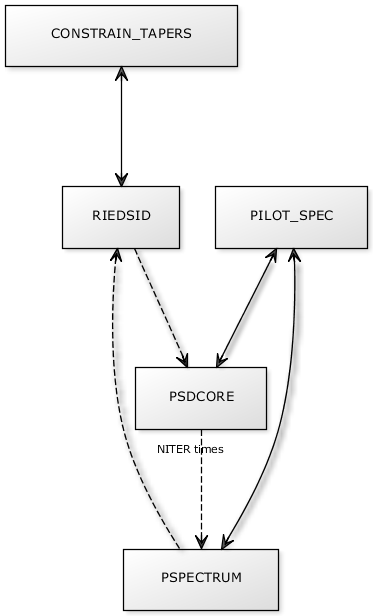
\includegraphics[width=0.5\textwidth]{yuml_d.png}%%
 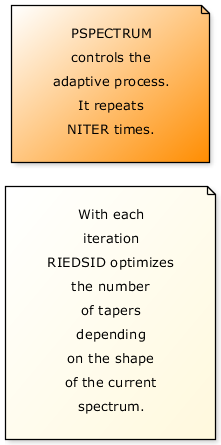
\includegraphics[width=0.3\textwidth]{yuml_n.png}
 \caption{Simplified call graph for \psd{}. The dashed lines show a
 simplified circuit
 which the spectra and its tapers make during the iterative process.}
 \label{fig:calls}
\end{figure}

\clearpage

\section*{Session Info}
\input{figure/SI.tex}

\clearpage

\bibliographystyle{apalike}
\bibliography{REFS}

\end{document}
